\documentclass[14pt]{extbook}
\usepackage{multicol, enumerate, enumitem, hyperref, color, soul, setspace, parskip, fancyhdr} %General Packages
\usepackage{amssymb, amsthm, amsmath, bbm, latexsym, units, mathtools} %Math Packages
\everymath{\displaystyle} %All math in Display Style
% Packages with additional options
\usepackage[headsep=0.5cm,headheight=12pt, left=1 in,right= 1 in,top= 1 in,bottom= 1 in]{geometry}
\usepackage[usenames,dvipsnames]{xcolor}
\usepackage{dashrule}  % Package to use the command below to create lines between items
\newcommand{\litem}[1]{\item#1\hspace*{-1cm}\rule{\textwidth}{0.4pt}}
\pagestyle{fancy}
\lhead{Progress Quiz 2}
\chead{}
\rhead{Version A}
\lfoot{7862-5421}
\cfoot{}
\rfoot{Spring 2021}
\begin{document}

\begin{enumerate}
\litem{
Solve the quadratic equation below. Then, choose the intervals that the solutions $x_1$ and $x_2$ belong to, with $x_1 \leq x_2$.\[ 25x^{2} +60 x + 36 = 0 \]\begin{enumerate}[label=\Alph*.]
\item \( x_1 \in [-1.49, 0.83] \text{ and } x_2 \in [-1.2, -1.17] \)
\item \( x_1 \in [-3.86, -3.58] \text{ and } x_2 \in [-0.5, -0.38] \)
\item \( x_1 \in [-2.65, -1.6] \text{ and } x_2 \in [-0.64, -0.53] \)
\item \( x_1 \in [-30.32, -29.07] \text{ and } x_2 \in [-30.19, -29.79] \)
\item \( x_1 \in [-7.7, -5.9] \text{ and } x_2 \in [-0.32, -0.16] \)

\end{enumerate} }
\litem{
Solve the quadratic equation below. Then, choose the intervals that the solutions $x_1$ and $x_2$ belong to, with $x_1 \leq x_2$.\[ 6x^{2} +35 x + 36 = 0 \]\begin{enumerate}[label=\Alph*.]
\item \( x_1 \in [-14.98, -13.29] \text{ and } x_2 \in [-0.47, -0.42] \)
\item \( x_1 \in [-2.74, -1.79] \text{ and } x_2 \in [-2.48, -2.19] \)
\item \( x_1 \in [-27.34, -26.41] \text{ and } x_2 \in [-8.28, -7.48] \)
\item \( x_1 \in [-9.19, -8.7] \text{ and } x_2 \in [-0.99, -0.57] \)
\item \( x_1 \in [-6.53, -4.35] \text{ and } x_2 \in [-2.24, -1.1] \)

\end{enumerate} }
\litem{
Write the equation of the graph presented below in the form $f(x)=ax^2+bx+c$, assuming  $a=1$ or $a=-1$. Then, choose the intervals that $a, b,$ and $c$ belong to.
\begin{center}
    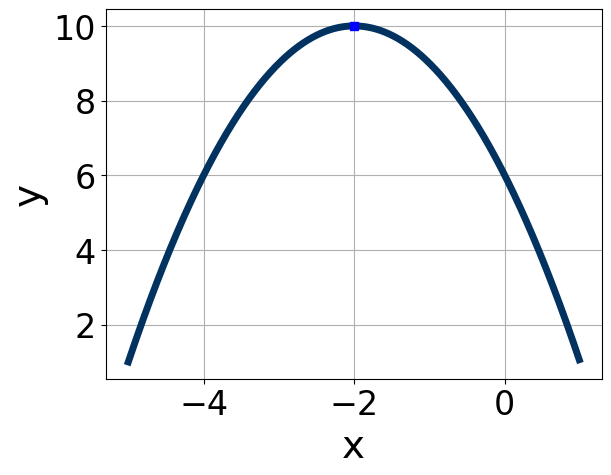
\includegraphics[width=0.5\textwidth]{../Figures/quadraticGraphToEquationCopyA.png}
\end{center}
\begin{enumerate}[label=\Alph*.]
\item \( a \in [1, 3], \hspace*{5mm} b \in [-6, -1], \text{ and } \hspace*{5mm} c \in [13, 15] \)
\item \( a \in [-1, 0], \hspace*{5mm} b \in [-6, -1], \text{ and } \hspace*{5mm} c \in [6, 10] \)
\item \( a \in [1, 3], \hspace*{5mm} b \in [2, 6], \text{ and } \hspace*{5mm} c \in [13, 15] \)
\item \( a \in [-1, 0], \hspace*{5mm} b \in [-6, -1], \text{ and } \hspace*{5mm} c \in [-14, -11] \)
\item \( a \in [-1, 0], \hspace*{5mm} b \in [2, 6], \text{ and } \hspace*{5mm} c \in [6, 10] \)

\end{enumerate} }
\litem{
Solve the quadratic equation below. Then, choose the intervals that the solutions belong to, with $x_1 \leq x_2$ (if they exist).\[ -12x^{2} +10 x + 4 = 0 \]\begin{enumerate}[label=\Alph*.]
\item \( x_1 \in [-0.5, 1.8] \text{ and } x_2 \in [0.5, 1.2] \)
\item \( x_1 \in [-16.8, -16.1] \text{ and } x_2 \in [16.8, 18.1] \)
\item \( x_1 \in [-15.3, -12.2] \text{ and } x_2 \in [2.3, 4.2] \)
\item \( x_1 \in [-2.7, -1] \text{ and } x_2 \in [-1.4, 0.7] \)
\item \( \text{There are no Real solutions.} \)

\end{enumerate} }
\litem{
Write the equation of the graph presented below in the form $f(x)=ax^2+bx+c$, assuming  $a=1$ or $a=-1$. Then, choose the intervals that $a, b,$ and $c$ belong to.
\begin{center}
    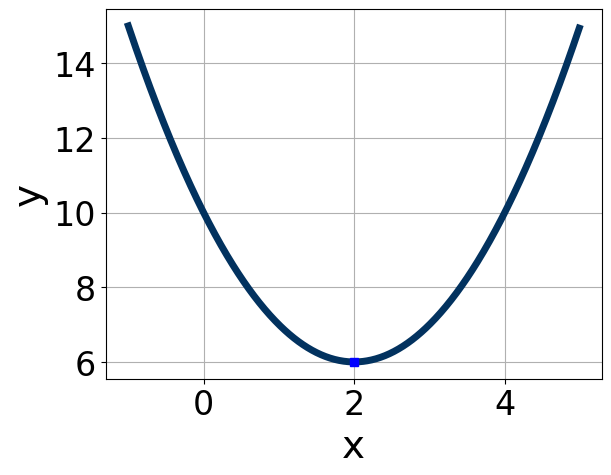
\includegraphics[width=0.5\textwidth]{../Figures/quadraticGraphToEquationA.png}
\end{center}
\begin{enumerate}[label=\Alph*.]
\item \( a \in [-3, 0], \hspace*{5mm} b \in [-9, -7], \text{ and } \hspace*{5mm} c \in [-6, -3] \)
\item \( a \in [1, 4], \hspace*{5mm} b \in [7, 10], \text{ and } \hspace*{5mm} c \in [26, 27] \)
\item \( a \in [1, 4], \hspace*{5mm} b \in [-9, -7], \text{ and } \hspace*{5mm} c \in [26, 27] \)
\item \( a \in [-3, 0], \hspace*{5mm} b \in [7, 10], \text{ and } \hspace*{5mm} c \in [-6, -3] \)
\item \( a \in [1, 4], \hspace*{5mm} b \in [7, 10], \text{ and } \hspace*{5mm} c \in [6, 11] \)

\end{enumerate} }
\litem{
Graph the equation below.\[ f(x) = (x-1)^2 + 11 \]\begin{enumerate}[label=\Alph*.]
\begin{multicols}{2}\item 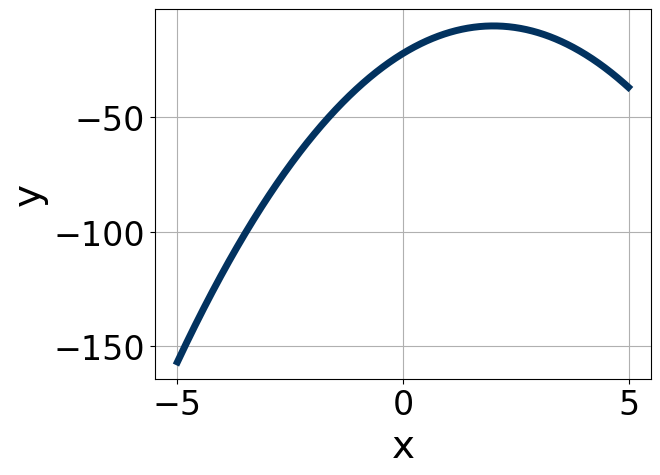
\includegraphics[width = 0.3\textwidth]{../Figures/quadraticEquationToGraphCopyAA.png}\item 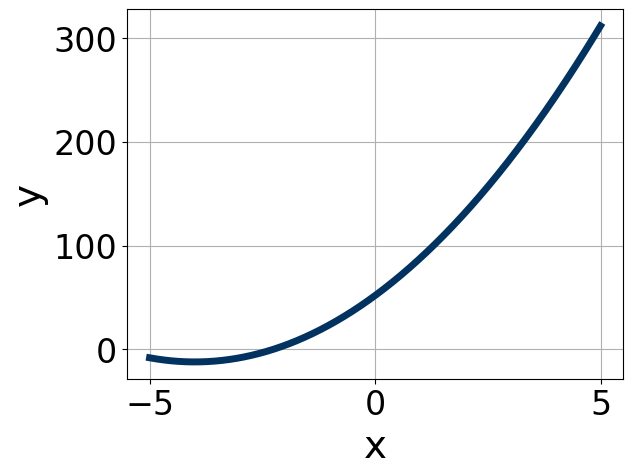
\includegraphics[width = 0.3\textwidth]{../Figures/quadraticEquationToGraphCopyBA.png}\item 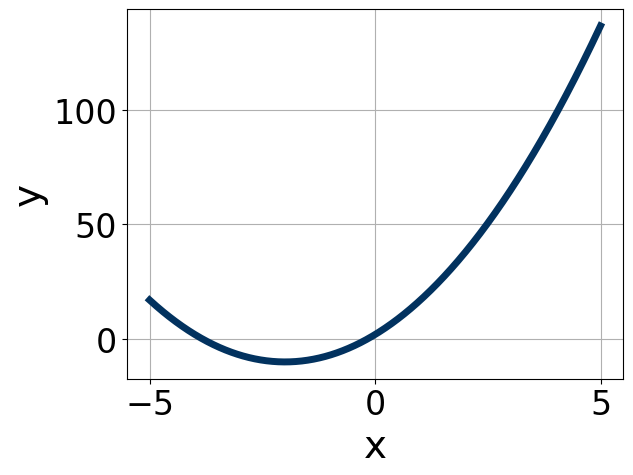
\includegraphics[width = 0.3\textwidth]{../Figures/quadraticEquationToGraphCopyCA.png}\item 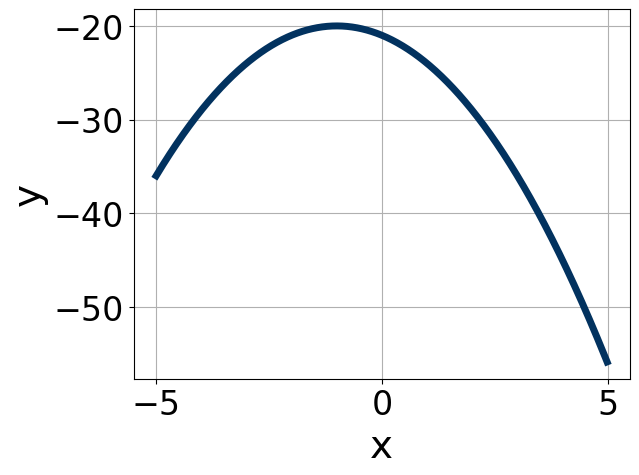
\includegraphics[width = 0.3\textwidth]{../Figures/quadraticEquationToGraphCopyDA.png}\end{multicols}\item None of the above.
\end{enumerate} }
\litem{
Graph the equation below.\[ f(x) = (x+3)^2 - 10 \]\begin{enumerate}[label=\Alph*.]
\begin{multicols}{2}\item 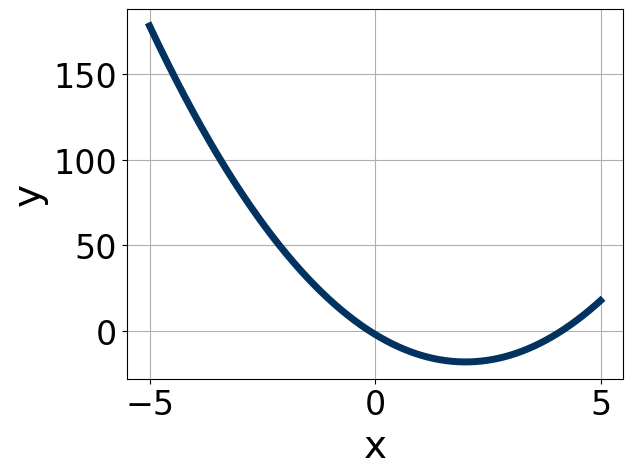
\includegraphics[width = 0.3\textwidth]{../Figures/quadraticEquationToGraphAA.png}\item 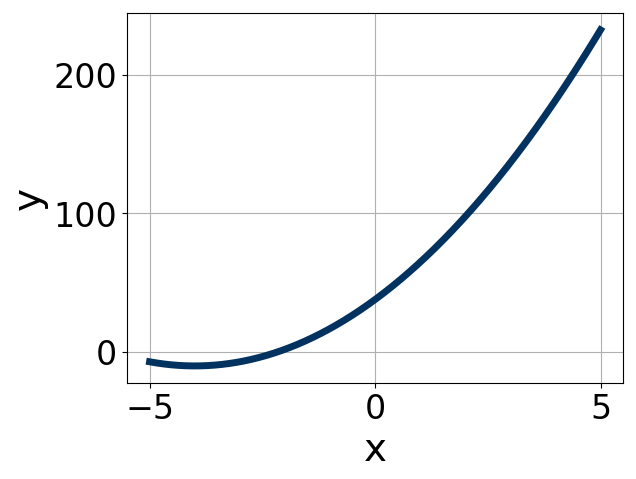
\includegraphics[width = 0.3\textwidth]{../Figures/quadraticEquationToGraphBA.png}\item 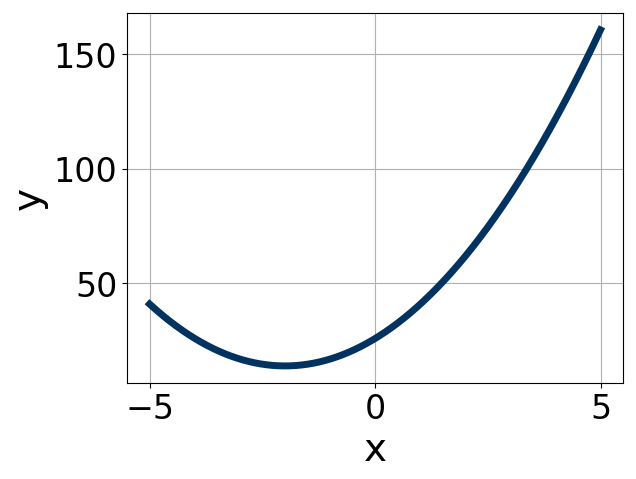
\includegraphics[width = 0.3\textwidth]{../Figures/quadraticEquationToGraphCA.png}\item 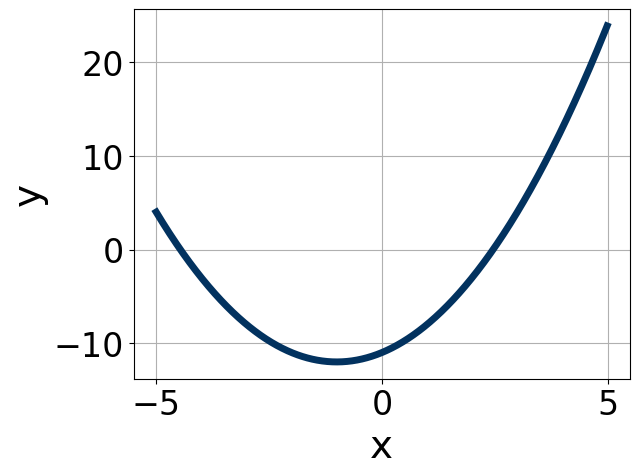
\includegraphics[width = 0.3\textwidth]{../Figures/quadraticEquationToGraphDA.png}\end{multicols}\item None of the above.
\end{enumerate} }
\litem{
Factor the quadratic below. Then, choose the intervals that contain the constants in the form $(ax+b)(cx+d); b \leq d.$\[ 36x^{2} -60 x + 25 \]\begin{enumerate}[label=\Alph*.]
\item \( a \in [-0.79, 1.47], \hspace*{5mm} b \in [-30, -29], \hspace*{5mm} c \in [0.13, 1.96], \text{ and } \hspace*{5mm} d \in [-32, -25] \)
\item \( a \in [3.63, 6.77], \hspace*{5mm} b \in [-5, -4], \hspace*{5mm} c \in [5.76, 6.62], \text{ and } \hspace*{5mm} d \in [-6, -2] \)
\item \( a \in [17.36, 19.3], \hspace*{5mm} b \in [-5, -4], \hspace*{5mm} c \in [1.52, 2.17], \text{ and } \hspace*{5mm} d \in [-6, -2] \)
\item \( a \in [1.58, 2.58], \hspace*{5mm} b \in [-5, -4], \hspace*{5mm} c \in [17.65, 18.57], \text{ and } \hspace*{5mm} d \in [-6, -2] \)
\item \( \text{None of the above.} \)

\end{enumerate} }
\litem{
Solve the quadratic equation below. Then, choose the intervals that the solutions belong to, with $x_1 \leq x_2$ (if they exist).\[ 16x^{2} +12 x -9 = 0 \]\begin{enumerate}[label=\Alph*.]
\item \( x_1 \in [-28.33, -26.99] \text{ and } x_2 \in [26.1, 26.55] \)
\item \( x_1 \in [-1.59, -0.66] \text{ and } x_2 \in [0.29, 0.57] \)
\item \( x_1 \in [-1.19, -0.15] \text{ and } x_2 \in [1.16, 1.71] \)
\item \( x_1 \in [-19.68, -19.03] \text{ and } x_2 \in [7.32, 7.75] \)
\item \( \text{There are no Real solutions.} \)

\end{enumerate} }
\litem{
Factor the quadratic below. Then, choose the intervals that contain the constants in the form $(ax+b)(cx+d); b \leq d.$\[ 24x^{2} +50 x + 25 \]\begin{enumerate}[label=\Alph*.]
\item \( a \in [11.14, 12.55], \hspace*{5mm} b \in [2, 11], \hspace*{5mm} c \in [1.45, 2.18], \text{ and } \hspace*{5mm} d \in [4, 9] \)
\item \( a \in [0.07, 1.03], \hspace*{5mm} b \in [11, 29], \hspace*{5mm} c \in [-0.41, 1.89], \text{ and } \hspace*{5mm} d \in [26, 34] \)
\item \( a \in [3.62, 4.44], \hspace*{5mm} b \in [2, 11], \hspace*{5mm} c \in [4.35, 6.84], \text{ and } \hspace*{5mm} d \in [4, 9] \)
\item \( a \in [1.1, 2.47], \hspace*{5mm} b \in [2, 11], \hspace*{5mm} c \in [11.34, 13.61], \text{ and } \hspace*{5mm} d \in [4, 9] \)
\item \( \text{None of the above.} \)

\end{enumerate} }
\end{enumerate}

\end{document}